% ---------------------------------------------------------------
% Figure: the disagreement-aware Probabilistic U-Net (training).
%
% Left/centre reproduces Fig. 1b of Kohl et al. (2018): encoders as stacks of
% blue blocks, latent spaces as Gaussian heatmaps, the sampled z as a green
% block WEDGED INSIDE the U-Net between the last decoder block and the final
% 1x1 block, prediction and ground truth side by side, and both long arrows
% entering the Posterior Net from opposite sides. Dashed box = our extension.
%
% Every coordinate here was checked numerically (no box overlaps, no line
% through a thumbnail or a label) and rendered to a raster preview before
% being committed. There is exactly ONE line-line crossing, at (16.00,-1.20):
% it is unavoidable, because the extension sits right of the grader masks so
% anything fed from the U-Net must cross the graders -> D^GT arrow.
% If you move something, keep the routes orthogonal and re-check by eye.
%
% The CT crop, the four grader masks and D^GT are REAL DATA, written by
%   python scripts/make_figure_assets.py
% from LIDC test crop LIDC-IDRI-0217 z-129.0_c0 into overleaf/figs/.
% The model's own outputs (y-hat, U, D-hat) are drawn as irregular schematic
% shapes, because no trained checkpoint exists yet -- they are NOT results.
% Once a model is trained, dump real maps and swap them in.
%
% Colour grammar: blue = network, green = loss, orange = added by us.
%
% Needs \usepackage{graphicx}, \usepackage{tikz}, \usetikzlibrary{arrows.meta}
% ---------------------------------------------------------------

\definecolor{pblue}{RGB}{198,219,239}
\definecolor{pgreen}{RGB}{45,125,60}
\definecolor{pours}{RGB}{214,96,20}

% Irregular closed curves, so the schematic maps do not read as clip art.
\newcommand{\blobpath}{plot[smooth cycle,tension=0.75] coordinates {%
  (0.25,0.00) (0.24,0.17) (0.10,0.32) (-0.10,0.29) (-0.19,0.14)
  (-0.35,0.00) (-0.25,-0.18) (-0.08,-0.25) (0.09,-0.28) (0.29,-0.21)}}
\newcommand{\ringpath}{plot[smooth cycle,tension=0.75] coordinates {%
  (0.36,0.00) (0.26,0.19) (0.09,0.28) (-0.09,0.26) (-0.32,0.23)
  (-0.26,0.00) (-0.24,-0.18) (-0.10,-0.31) (0.11,-0.33) (0.19,-0.14)}}

% Three visibly DIFFERENT shapes for the K prior samples. They must not be
% copies of one another: the whole point of the sample stack is that the model
% produces diverse segmentations.
\newcommand{\sampleApath}{plot[smooth cycle,tension=0.75] coordinates {%
  (0.34,0.00) (0.26,0.19) (0.07,0.23) (-0.10,0.30) (-0.29,0.21)
  (-0.26,0.00) (-0.22,-0.16) (-0.11,-0.34) (0.09,-0.28) (0.20,-0.15)}}
\newcommand{\sampleBpath}{plot[smooth cycle,tension=0.75] coordinates {%
  (0.24,0.00) (0.25,0.18) (0.08,0.23) (-0.07,0.21) (-0.24,0.18)
  (-0.28,0.00) (-0.17,-0.12) (-0.09,-0.26) (0.09,-0.29) (0.18,-0.13)}}
\newcommand{\sampleCpath}{plot[smooth cycle,tension=0.75] coordinates {%
  (0.35,0.00) (0.23,0.17) (0.10,0.31) (-0.13,0.39) (-0.22,0.16)
  (-0.31,0.00) (-0.31,-0.22) (-0.10,-0.32) (0.08,-0.24) (0.32,-0.23)}}

% a segmentation-like map: x, y, half-size, shape scale, path macro
\newcommand{\blobmap}[5]{%
  \begin{scope}[shift={(#1,#2)}]
    \fill[black] (-#3,-#3) rectangle (#3,#3);
    \begin{scope}[scale=#4] \fill[white] #5; \end{scope}
    \draw[black!55,line width=0.4pt] (-#3,-#3) rectangle (#3,#3);
  \end{scope}}
% a map peaked on the lesion boundary (U, D-hat): x, y
\newcommand{\ringmap}[2]{%
  \begin{scope}[shift={(#1,#2)}]
    \fill[black] (-0.6,-0.6) rectangle (0.6,0.6);
    % Thick enough to read as a heat-map rim like the real D^GT beside it, not
    % as a thin outline -- the reader is meant to compare U and D-hat to D^GT.
    \draw[line width=4.2pt,red!70!black]    \ringpath;
    \draw[line width=2.4pt,orange!90!black] \ringpath;
    \draw[line width=1.0pt,yellow!85!white] \ringpath;
    \draw[black!55,line width=0.4pt] (-0.6,-0.6) rectangle (0.6,0.6);
  \end{scope}}
% a latent space: Gaussian blob. x, y, half-size
\newcommand{\latentmap}[3]{%
  \begin{scope}[shift={(#1,#2)}]
    \fill[black!55] (-#3,-#3) rectangle (#3,#3);
    \fill[black!38] (0,0) ellipse (0.40 and 0.32);
    \fill[black!22] (0,0) ellipse (0.28 and 0.22);
    \fill[black!8]  (0,0) ellipse (0.15 and 0.12);
    \draw[black!55,line width=0.4pt] (-#3,-#3) rectangle (#3,#3);
  \end{scope}}

% [!ht] not [t]: the figure plus its caption is ~two thirds of a text block, so
% plain [t] fails LaTeX's size test on every page and gets deferred to the end,
% four pages after the text that references it. The ! overrides those limits.
\begin{figure}[!ht]
\centering
\resizebox{\textwidth}{!}{%
\begin{tikzpicture}[
  font=\footnotesize,
  >={Stealth[length=2mm]},
  fm/.style    ={fill=pblue,draw=black!45,line width=0.3pt},
  pic/.style   ={draw=black!55,inner sep=0pt,line width=0.4pt},
  flow/.style  ={->,draw=black!65,thick},
  oflow/.style ={->,draw=pours,thick},
  loss/.style  ={<->,draw=pgreen,very thick},
  lbl/.style   ={font=\scriptsize,inner sep=1.5pt},
  olbl/.style  ={font=\scriptsize,text=pours,inner sep=1.5pt},
]

% dashed region first, so it sits behind everything
\draw[pours,thick,dashed,rounded corners=3pt] (14.40,-4.55) rectangle (20.55,2.20);
\node[olbl,font=\small\bfseries] at (17.45,2.42) {ours};

% ============ ORIGINAL PROBABILISTIC U-NET ============
\node[pic] at (3.40,-1.20) {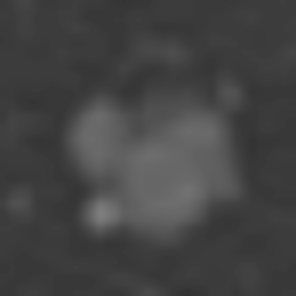
\includegraphics[width=12mm]{figs/ct}};
\node[lbl] at (3.40,-2.05) {Image};

\fill[fm] (4.45,0.85) rectangle (4.61,1.75);
\fill[fm] (4.73,0.98) rectangle (4.89,1.62);
\fill[fm] (5.01,1.08) rectangle (5.17,1.52);
\node[lbl] at (4.81,0.60) {Prior Net};

\latentmap{6.60}{1.30}{0.7}
\node[lbl] at (6.60,0.42) {$p(z\mid x)$};
\latentmap{9.00}{1.30}{0.7}
\node[lbl,anchor=west] at (8.70,0.42) {$q(z\mid x,Y_g)$};

\fill[fm] (8.56,3.00) rectangle (8.72,3.80);
\fill[fm] (8.92,3.08) rectangle (9.08,3.72);
\fill[fm] (9.28,3.15) rectangle (9.44,3.65);
\node[lbl] at (9.00,4.05) {Posterior Net};

% U-Net: encoder down, decoder up, sampled z (green) wedged between the last
% decoder block and the final 1x1 block, exactly as in the paper.
\fill[fm] (5.66,-1.50) rectangle (5.82,-0.30);
\fill[fm] (6.06,-1.70) rectangle (6.22,-0.80);
\fill[fm] (6.46,-1.85) rectangle (6.62,-1.25);
\fill[fm] (6.86,-2.00) rectangle (7.14,-1.60);
\fill[fm] (7.38,-1.85) rectangle (7.54,-1.25);
\fill[fm] (7.78,-1.70) rectangle (7.94,-0.80);
\fill[fm] (8.18,-1.50) rectangle (8.34,-0.30);
\fill[pgreen!35,draw=black!45,line width=0.3pt] (8.34,-1.50) rectangle (8.50,-0.30);
\fill[fm] (8.50,-1.50) rectangle (8.66,-0.30);
\draw[->,blue!55!black,line width=0.4pt] (5.82,-0.45) -- (8.18,-0.45);
\draw[->,blue!55!black,line width=0.4pt] (6.22,-0.90) -- (7.78,-0.90);
\draw[->,blue!55!black,line width=0.4pt] (6.62,-1.35) -- (7.38,-1.35);
\node[lbl] at (7.20,-2.15) {U-Net};

\blobmap{10.90}{-1.20}{0.6}{1.0}{\blobpath}
\node[lbl,align=center] at (10.90,-2.13) {Predicted\\segmentation};

% the four graders; the one drawn at random as Y_g is outlined in green
\node[pic] at (12.90,-0.88) {
\includegraphics[width=6mm]{figs/mask0}};
\node[pic] at (13.52,-0.88) {
\includegraphics[width=6mm]{figs/mask1}};
\node[pic] at (12.90,-1.50) {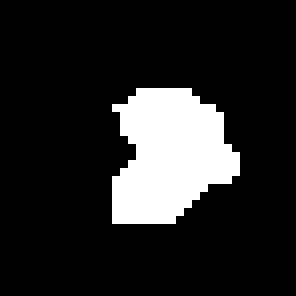
\includegraphics[width=6mm]{figs/mask2}};
\node[pic] at (13.52,-1.50) {
\includegraphics[width=6mm]{figs/mask3}};
\draw[pgreen,line width=1.1pt] (12.60,-1.18) rectangle (13.20,-0.58);
\node[lbl] at (13.21,-2.08) {$Y_1..Y_4$};

% one trunk out of the image, branching to the Prior Net
\draw[flow] (3.40,-0.60) -- (3.40,2.60) -- (8.20,2.60) -- (8.20,3.40) -- (8.56,3.40);
\draw[flow] (3.40,1.30) -- (4.45,1.30);
\draw[flow] (4.00,-1.20) -- (5.66,-1.20);
\draw[flow] (5.17,1.30) -- (5.90,1.30);
\draw[flow] (9.00,3.08) -- (9.00,2.00);
\draw[loss] (7.30,1.30) -- (8.30,1.30);
\node[lbl] at (7.80,1.48) {KL};
\draw[flow] (8.42,0.60) -- (8.42,-0.30);
\node[lbl,anchor=east] at (8.34,0.04) {Sample $z$};
\draw[flow] (8.66,-1.20) -- (10.30,-1.20);
\draw[loss] (11.50,-1.20) -- (12.60,-1.20);
\node[lbl] at (12.05,-0.32) {cross-entropy};
\draw[flow] (13.21,-0.58) -- (13.21,3.40) -- (9.44,3.40);

% ============ OUR EXTENSION ============
% Side by side, NOT a diagonal stack: overlapping tiles hide the shapes behind
% them, and the whole point of showing several is that they visibly differ.
\blobmap{15.42}{0.90}{0.28}{0.70}{\sampleApath}
\blobmap{16.00}{0.90}{0.28}{0.70}{\sampleBpath}
\blobmap{16.58}{0.90}{0.28}{0.70}{\sampleCpath}
\node[olbl] at (16.00,1.50) {$Q^{(1)},\dots,Q^{(K)}$};

\ringmap{18.80}{0.90}
\node[lbl,anchor=west] at (19.50,0.90) {$U$};

\node[pic] at (18.80,-1.20) {
\includegraphics[width=12mm]{figs/dgt}};
\node[lbl,anchor=west] at (19.50,-1.20) {$D^{GT}$};

\draw[pours,thick,rounded corners=2pt,fill=pours!8]
      (14.95,-3.75) rectangle (17.05,-3.05);
\node[lbl] at (16.00,-3.40) {$1{\times}1$ conv $+\ \sigma$};

\ringmap{18.80}{-3.40}
\node[lbl,anchor=west] at (19.50,-3.40) {$\hat D$};

% F(x) taps the decoder BEFORE z is injected, so it keeps the deeper lane and
% never has to cross the branch that re-runs the network with prior samples.
\draw[oflow] (8.26,-1.50) -- (8.26,-3.40) -- (14.95,-3.40);
\node[olbl] at (11.60,-3.66) {$F(x)$, before $z$};
% NOTE: these K passes re-run the network with z drawn from the PRIOR, not the
% posterior z that produced the prediction above. Labelled on the arrow itself,
% because the arrow leaves the decoder and would otherwise imply the same z.
\draw[oflow] (8.58,-1.50) -- (8.58,-2.50) -- (16.00,-2.50) -- (16.00,0.62);
\node[olbl] at (12.00,-2.72) {$K$ passes with $z_k\sim p(z\mid x)$};
\draw[oflow] (13.82,-1.20) -- (18.20,-1.20);
\draw[oflow] (16.86,0.90) -- (18.20,0.90);
\draw[oflow] (17.05,-3.40) -- (18.20,-3.40);

\draw[loss] (18.80,0.30) -- (18.80,-0.60);
\node[lbl,anchor=east] at (18.65,-0.15) {$L_{\text{align}}$};
\draw[loss] (18.80,-2.80) -- (18.80,-1.80);
\node[lbl,anchor=east] at (18.65,-2.30) {$L_D$};

\end{tikzpicture}}
% Kept deliberately short: Section 2 already states the method, so the caption
% only orients the reader and records the two things the drawing encodes that
% the text cannot show. Resist re-expanding it -- figure + caption is already
% about two thirds of a text block.
\caption{\textbf{The disagreement-aware Probabilistic U-Net (training).}
Outside the dashed box, the original model: its posterior sees the image and
\emph{one} randomly drawn grader $Y_g$ (green outline), and its sampled $z$
(green block) enters the decoder before the final $1{\times}1$ convolutions.
Inside, our extension. $D^{GT}$ --- the normalized binary entropy of the four
graders' per-pixel mean --- peaks in a rim where they disagree; we supervise
$\hat D$ against it with $L_D$ (MSE) and $U$ with $L_{\text{align}}$ ($\ell_1$),
the term that places predictive diversity where annotators actually disagree.
Two things the drawing encodes: $F(x)$ is tapped \emph{before} $z$, so $\hat D$
depends on the image alone; and the $K$ passes behind $U$ draw fresh $z_k$ from
the \emph{prior}, not the posterior $z$ that produced the prediction. The CT
crop, the four masks and $D^{GT}$ are real data (\texttt{LIDC-IDRI-0217});
the predicted segmentation, $U$ and $\hat D$ are schematic, and feature-map
blocks are reduced for clarity.}
\label{fig:model}
\end{figure}
